\documentclass{article}
\usepackage[margin=1in]{geometry}
\usepackage{amsmath}
\usepackage{graphicx}
\usepackage{siunitx}
\usepackage{listings}
\usepackage{xcolor}
\usepackage{hyperref}
\definecolor{mygreen}{rgb}{0,0.6,0}
\definecolor{mygray}{rgb}{0.5,0.5,0.5}
\definecolor{mymauve}{rgb}{0.58,0,0.82}

\lstset{ %
  backgroundcolor=\color{white},   % choose the background color; you must add \usepackage{color} or \usepackage{xcolor}
  basicstyle=\scriptsize\ttfamily,    % the size of the fonts that are used for the code
  breakatwhitespace=false,         % sets if automatic breaks should only happen at whitespace
  breaklines=true,                 % sets automatic line breaking
  captionpos=b,                    % sets the caption-position to bottom
  commentstyle=\color{mygreen},    % comment style
  deletekeywords={},            % if you want to delete keywords from the given language
  escapeinside={\%*}{*)},          % if you want to add LaTeX within your code
  extendedchars=true,              % lets you use non-ASCII characters; for 8-bits encodings only, does not work with UTF-8
  frame=shadowbox,                    % adds a frame around the code
%  framexleftmarign=5mm,
  xleftmargin=10pt,
  xrightmargin=10pt,
  rulesepcolor=\color{gray},
  keywordstyle=\color{blue},       % keyword style
  language=Octave,                 % the language of the code
  morekeywords={*,...,fit,predint,export\_fig},            % if you want to add more keywords to the set
%  numbers=left,                    % where to put the line-numbers; possible values are (none, left, right)
  numbers=none,
  numbersep=5pt,                   % how far the line-numbers are from the code
  numberstyle=\tiny\color{mygray}, % the style that is used for the line-numbers
  rulecolor=\color{black},         % if not set, the frame-color may be changed on line-breaks within not-black text (e.g. comments (green here))
  showspaces=false,                % show spaces everywhere adding particular underscores; it overrides 'showstringspaces'
  showstringspaces=false,          % underline spaces within strings only
  showtabs=false,                  % show tabs within strings adding particular underscores
  stepnumber=1,                    % the step between two line-numbers. If it's 1, each line will be numbered
  stringstyle=\color{mymauve},     % string literal style
  tabsize=4,                       % sets default tabsize to 4 spaces
  caption=\lstname                   % show the filename of files included with \lstinputlisting; also try caption instead of title
}


\title{1.723 HW3}
\author{Sachith  Dunatunga}

\begin{document}
\maketitle

\section{Problem 1}
\subsection{Part 1}
The equation we want to nondimensionalize is given by
\begin{align}
    c_t \frac{\partial p}{\partial t} + \frac{\partial}{\partial x} \left( \frac{-k}{\mu} \frac{\partial p}{\partial x} \right) = 0.
    \label{eqn:pressure}
\end{align}

We note first that all the variables can be written as $x_D = x / x_c$, $p_D = p / p_c$, and etc.
Moreover, the derivatives are given by $dx_D = dx / x_c$, $dp_D = dp / p_c$, and etc.

Using the chain rule, we can then rewrite equation \eqref{eqn:pressure} as
\begin{align}
    \frac{c_t p_c}{T_c} \frac{\partial p_D}{\partial t_D} + \frac{1}{x_c} \frac{\partial}{\partial x_D} \left( \frac{-k_D k_c}{\mu_D \mu_c} \frac{p_c}{x_c} \frac{\partial p_D}{\partial x_D} \right) = 0
\end{align}
which can be rearranged into
\begin{align}
    \frac{c_t p_c}{T_c} \frac{\partial p_D}{\partial t_D} + \frac{k_c p_c}{x_c^2 \mu_c} \frac{\partial}{\partial x_D} \left( \frac{-k_D}{\mu_D}\frac{\partial p_D}{\partial x_D} \right) = 0.
\end{align}
The coefficients can be collected together into
\begin{align}
    \frac{\partial p_D}{\partial t_D} + \frac{T_c k_c}{c_t x_c^2 \mu_c} \frac{\partial}{\partial x_D} \left( \frac{-k_D}{\mu_D}\frac{\partial p_D}{\partial x_D} \right) = 0.
\end{align}

Setting the term
\begin{align}
    \frac{T_c k_c}{c_t x_c^2 \mu_c}
\end{align}
to unity yields the expression
\begin{align}
    T_c = \frac{c_t x_c^2 \mu_c}{k_c} = \frac{c_t L^2 \mu_c}{k_c}
\end{align}

\subsection{Part 2}
The Darcy velocity is given by
\begin{align}
\mathbf{u} = \frac{-k}{\mu} \nabla p.
\end{align}
In 1D we have
\begin{align}
u = \frac{-k}{\mu} \frac{\partial p}{\partial x}.
\end{align}
Following the same procedure as the time, we arrive at
\begin{align}
u_c u_D = \frac{-k_c k_D}{\mu_c \mu_D} \frac{p_c}{x_c} \frac{\partial p_D}{\partial x_D},
\end{align}
and after collecting terms and substituting we have
\begin{align}
u_c = \frac{k_c p_c}{\mu_c L}.
\end{align}

\subsection{Part 3}
We calculate the above quantities given
\begin{align}
    L &= \num{1e3}\ \si{\meter} \\
    k_c &= \num{1e-13}\ \si{\meter\squared} \\
    \mu_c &= \num{1e-3}\ \si[inter-unit-product = \ensuremath{{}\cdot{}}]{\pascal\second} \\
    c_t &= \num{1e-8}\ \si{\per\pascal} \\
    \Delta P_c &= \num{1e5}\ \si{\pascal}.
\end{align}

Plugging in yields
\begin{align}
    T_c = \frac{c_t L^2 \mu_c}{k_c} = \frac{10^{-8} (10^3)^2 10^{-3}}{10^{-13}}\ \si{\second} = 10^8\ \si{\second}
\end{align}
(which seems a bit long at approximately 3 years) and
\begin{align}
    u_c = \frac{k_c p_c}{\mu_c L} = \frac{10^{-13} 10^5}{10^{-3} 10^3} = 10^{-8}\ \si{\meter\per\second}.
\end{align}


\section{Problem 2}
\subsection{Part 1}

We want to solve the nondimensionalized equation
\begin{align}
    \frac{\partial p}{\partial t} + \frac{\partial}{\partial x} \left( -\lambda \frac{\partial p}{\partial x} \right) = 0
\end{align}
(with $\lambda = 1$) subject to the boundary conditions
\begin{align}
    p(0, t) &= 1 \\
    -\lambda \frac{\partial p}{\partial x}\bigg\rvert_{x=1} &= 0
\end{align}
for $t > 0$ and initial condition
\begin{align}
p(x, 0) = 0.
\end{align}

We note that the boundary conditions are not homogenous.
We first calculate the steady state solution $p_s(x)$ given by
\begin{align}
    \frac{\partial^2 p_s}{\partial x^2} = 0
\end{align}
with boundary conditions
\begin{align}
    p_s(0) &= 1 \\
    -\frac{\partial p_s}{\partial x}\bigg\rvert_{x=1} &= 0.
\end{align}
The general solution is found by integrating twice to obtain
\begin{align}
    p_s(x) = Ax + B.
\end{align}
Using the BCs we obtain $p_s(0) = B = 1$ and $p_s'(1) = A = 0$, so the steady state solution is the constant $p_s(x) = 1$.

We now transform the equation for $p(x,t)$ to an equation for $p_t(x,t)$ given by $p(x,t) = p_t(x,t) + p_s(x)$.
Plugging in and substituting yields
\begin{align}
    \frac{\partial p_t}{\partial t} + \frac{\partial}{\partial x} \left( - \frac{\partial p_t}{\partial x} \right) = 0
    \label{eqn:p-transient}
\end{align}
with boundary conditions
\begin{align}
    p_t(0, t) &= 0 \\
    -\frac{\partial p_t}{\partial x}\bigg\rvert_{x=1} &= 0
\end{align}
(which are homogenous) and initial condition
\begin{align}
    p_t(x, 0) = -1.
\end{align}

We solve equation \eqref{eqn:p-transient} by using separation of variables. Assume we can decompose as $p_t(x,t) = X(x)T(t)$.
We then arrive at the equation
\begin{align}
    X(x)T'(t) - T(t)X''(x) = 0,
\end{align}
which can be expressed as the pair of equations
\begin{align}
    \frac{X''(x)}{X(x)} = \frac{T'(t)}{T(t)} = -\omega^2
\end{align}
We can use the characteristic roots to obtain the general solutions $X(x) = A\sin(\omega x) + B\cos(\omega x)$ and $T(t) = C\exp(-\omega^2 t)$, where $A$, $B$, and $C$ are arbitrary constants.
Without loss of generality we can absorb the constant $C$ to obtain the general solution for $p_t(x,t) = (\tilde{A}\sin(\omega x) + \tilde{B}\cos(\omega x))\exp(-\omega^2 t)$.
This solution must satisfy the boundary conditions, so we know that
\begin{align}
    p_t(0, t) &= 0 \\
    \tilde{B} \exp(-\omega^2 t) &= 0 \implies \tilde{B} = 0
\end{align}
and
\begin{align}
    -\frac{\partial p_t}{\partial x}\bigg\rvert_{x=1} &= 0 \\
    \tilde{A}\omega \cos(\omega) &= 0.
\end{align}
Since we don't want the trivial solution (when $\tilde{A} = 0$), we instead set $\cos(\omega) = 0$ by forcing special values of $\omega$.
In this case, we want $\omega = \frac{\pi}{2} (2n - 1)$ where $n$ is a whole number.
This generates a new solution for each $\omega$, which each satisfy the (homogenous) PDE, so we can sum them together and still get a solution.
Thus, we can write
\begin{align}
    p_t(x,t) = \sum_{n=1}^{\infty} a_n \sin\left(\frac{\pi}{2} (2n - 1) x\right) \exp\left(-\frac{\pi^2}{4} (2n - 1)^2 t \right)
\end{align}

We determine the $a_n$ by first noting that
\begin{align}
    \int_0^1 \sin\left(\frac{\pi}{2} (2n - 1) x\right) \sin\left(\frac{\pi}{2} (2m - 1) x\right) \mathrm{dx} = \frac{1}{2} \delta_{mn}
\end{align}
where $\delta_{mn} = 1$ if $m = n$ and $0$ otherwise.
The orthogonality of the sines allows us to determine $a_n$ by simply integrating the initial conditions against the corresponding sine function, yielding
\begin{align}
a_n &= 2 \int_0^1 (-1) \sin\left(\frac{\pi}{2} (2n - 1) x\right) \mathrm{dx} \\
    &= -2 \frac{2}{\pi (2n - 1)} \cos\left(\frac{\pi}{2} (2n - 1) x\right) \bigg\rvert_{x=0}^{x=1} \\
a_n &= \frac{-4}{\pi (2n - 1)}.
\end{align}

The complete solution for $p_t(x,t)$ is then
\begin{align}
    p_t(x,t) = \sum_{n=1}^{\infty} \frac{-4}{\pi (2n - 1)} \sin\left(\frac{\pi}{2} (2n - 1) x\right) \exp\left(-\frac{\pi^2}{4} (2n - 1)^2 t \right)
\end{align}
and likewise $p(x,t) = p_t(x,t) + p_s(x)$ is given by
\begin{align}
    p(x,t) = 1 + \sum_{n=1}^{\infty} \frac{-4}{\pi (2n - 1)} \sin\left(\frac{\pi}{2} (2n - 1) x\right) \exp\left(-\frac{\pi^2}{4} (2n - 1)^2 t \right)
\end{align}

When numerically evaulating this, we note that increasing $n$ results in a smaller contribution to the total solution, since each term has at least an $\exp\left(-\frac{\pi^2}{4} (2n - 1)^2 t \right)$ factor and sine is bounded to have a magnitude of 1 at most.
Moreover, the $a_n$ have a maximum magnitude of $-4/\pi$ at $n=1$.
This means we can conservatively estimate the maximum contribution of term $n$ as the exponential part alone.
If we are given a time $t$, we can ensure that no term beyond $n$ contributes more than $\epsilon$ error when we reach term
\begin{align}
n_{\mathrm{max}} = \Bigg\lceil \frac{1}{2}\left(1 + \frac{2}{\pi} \sqrt{\frac{-\log{\epsilon}}{t}}\right) \Bigg\rceil
\end{align}
and moreover this converges quickly since each term is exponentially smaller than the previous one.
We also can sum in reverse order (that is down from $n_{\mathrm{max}}$ to 1, essentially from small to large terms) to prevent too much error in the naive summation.
We implemented both the cutoff and the reverse sum in the plotting code used to generate figure \ref{fig:p_analytic}.

Due to the exponential, it doesn't take long to get close to the steady state.
Even by $t=2.0$, the solution is nearly indistinguishable from the steady state case.

\begin{figure}[!ht]
    \centering
    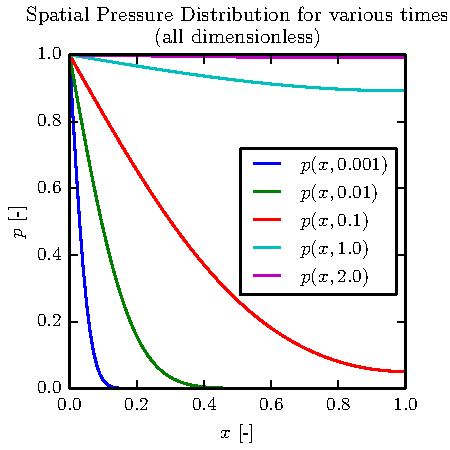
\includegraphics[scale=1.0]{p_over_time.pdf}
    \caption{The nondimensional pressure distribution $p(x,t)$ is plotted at various nondimensional times.
    We see that even by $t=2.0$, the solution is almost completely at the steady-state solution of $p(x,t) = 1$.}
    \label{fig:p_analytic}
\end{figure}

\subsection{Part 2}
For the spatial discretization we use the cell-centered finite volume method.
This means that the solution $p_i$ exists at locations $x_i = i*h + h/2$ where $h = 1/N$, $N$ the number of grid points.
The next flux for each cell is given by
\begin{align}
    \frac{\partial p}{\partial t} = -\frac{F_{i+1/2} - F_{i-1/2}}{h}.
\end{align}
The $F_{i \pm 1/2}$ are in turn given by
\begin{align}
    F_{i + 1/2} &= \frac{p_{j+1} - p_j}{h} \\
    F_{i - 1/2} &= \frac{p_{j} - p_{j-1}}{h}.
\end{align}

We use the trapezoidal rule in time, which is given by
\begin{align}
   p_n^{t+1} = p_n^{t} + \Delta t \left( \theta f(p^{t+1}) + (1 - \theta) f(p^{t}) \right)
\end{align}

Combining yields the following rule, applicable to interior points
\begin{align}
   p_n^{t+1} = p_n^{t} + \frac{\Delta t}{h^2}\left( (p_{n+1}^{t+1} - 2p_n^{t+1} + p_{n-1}^{t+1}) \theta +  (p_{n+1}^{t} - 2p_n^{t} + p_{n-1}^{t}) (1 - \theta) \right)
\end{align}

For boundaries, we must determing the value of the ghost point to enforce the BC and build it into the equation.
For the left side, we want the dirichlet BC $p(0,t) = 1$.
Averaging the cell centers achieves this; if $p_1$ is the leftmost cell center in the computational domain, $p_0$ is the ghost point.
The boundary condition is then
\begin{align}
    \frac{1}{2}(u_0 + u_1) = 1 \implies u_0 = 2 - u_1,
\end{align}
which is the substituted into the general form to obtain
\begin{align}
    p_1^{t+1} = p_1^{t} + \frac{\Delta t}{h^2}\left( (p_{2}^{t+1} - 3p_n^{t+1} + 2) \theta +  (p_{2}^{t} - 3p_1^{t} + 2) (1 - \theta) \right)
\end{align}

The right boundary (after $p_4$) is given by a zero slope condition, which is equivalent to setting the flux term to zero, which gives
\begin{align}
    F_{9/2} = 0 \implies -p_4 = p_5.
\end{align}
This is also substituted into the general form, which yields
\begin{align}
   p_4^{t+1} = p_4^{t} + \frac{\Delta t}{h^2}\left( (p_{5}^{t+1} - p_4^{t+1}) \theta +  (p_{5}^{t} - p_4^{t}) (1 - \theta) \right).
\end{align}

With the boundary conditions, interior points, and initial condition (given by the zero vector), we have enough information to simulate the system.

First we define the matrix $\mathbf{A}$ by
\begin{align}
    \mathbf{A} = \frac{\Delta t}{h^2} \begin{bmatrix}
                    -3 & 1 & 0 & 0 \\
                    1 & -2 & 1 & 0 \\
                    0 & 1 & -2 & 1 \\
                    0 & 0 & 1 & -1
                \end{bmatrix},
\end{align}
and the additional load vector $\tilde{\mathbf{p}}$ as
\begin{align}
\tilde{\mathbf{p}} = \frac{\Delta t}{h^2} \begin{bmatrix}
                    2 \\
                    0 \\
                    0 \\
                    0
                    \end{bmatrix}.
\end{align}

The system of equations is then written as
\begin{align}
    (\mathbf{I} - \theta \mathbf{A}) \mathbf{p}^{t+1} = (\mathbf{I} - (1 - \theta) \mathbf{A}) \mathbf{p}^t + \tilde{\mathbf{p}}
\end{align}
Where $\mathbf{I}$ is the identity matrix (4 by 4 in this case).
Note also that $p^{t+1} = p^{t+\Delta t}$. This is equivalent to the matrix equation
\begin{align}
    \tilde{\mathbf{A}} \tilde{\mathbf{x}} = \tilde{\mathbf{b}}
\end{align}
where the unknowns $\tilde{\mathbf{x}} = \mathbf{p}^{t+1}$, the matrix $\tilde{\mathbf{A}} = \mathbf{I} - \theta \mathbf{A}$, and the load $\tilde{\mathbf{b}} = (\mathbf{I} - (1 - \theta) \mathbf{A}) \mathbf{p}^t + \tilde{\mathbf{p}}$.


\subsection{Part 3}
The code is attached, but I will reproduce it here as well (I am sorry, but I did not have access to MATLAB since I am away at APS March Meeting, so I used python instead).
\lstinputlisting[label=code:integrate]{integrate_pressure.py}

\subsection{Part 4}
The numerical integration is very close to the analytical solutions, so I will instead plot the difference $p_{\mathrm{numeric}}(x,t_n) - p_{\mathrm{analytic}}(x,t_n)$ for various $t_n$.

\begin{tabular}{c c}
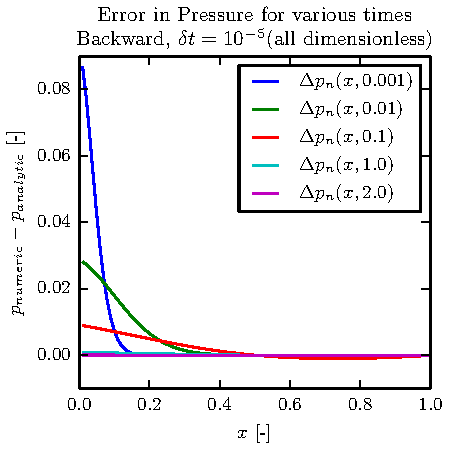
\includegraphics[scale=1.0]{error_backward_small.pdf} &
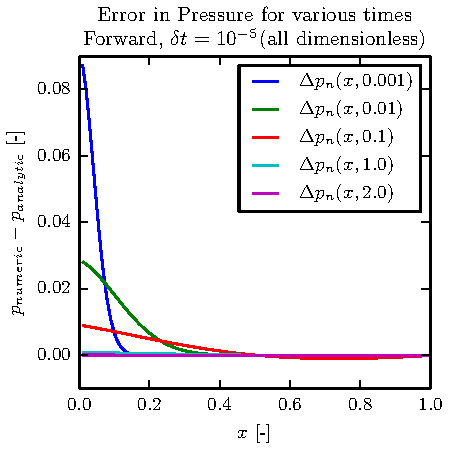
\includegraphics[scale=1.0]{error_forward_small.pdf}
\end{tabular}

As shown above, the error is fairly small for both methods. However, in terms of computational time, the forward method takes much less time because there is no matrix inversion done.

\subsection{Part 5}
It appears that the Forward Euler ($\theta = 0$) scheme is unstable, as the solution quickly develops oscillations and is not able to continue for long after that.
We can see this from the plots of error below (values not drawn are infinite).

\begin{tabular}{c c}
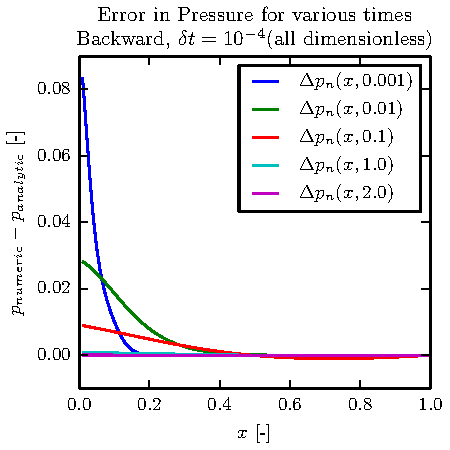
\includegraphics[scale=1.0]{error_backward_large.pdf} &
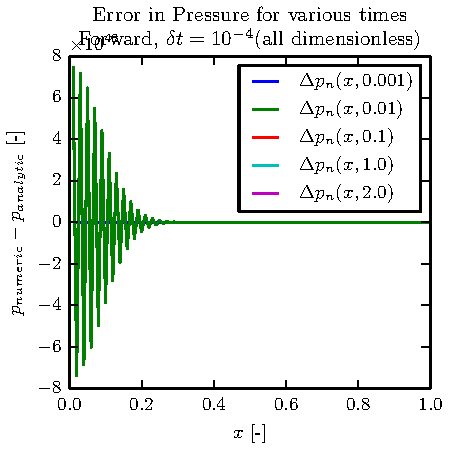
\includegraphics[scale=1.0]{error_forward_large.pdf}
\end{tabular}

This is because we have violated the CFL condition, which states that a function of timestep and grid size must not exceed a critical value.
For diffusion problems this is formulated as $\Delta t  / h^2 < C$.
The backward euler method suffers a bit in accuracy, but it remains stable.
The computational time remains large in comparision to the forward method, though this is no surprise.


% \appendix
% \section{Programs}
% \lstinputlisting[label=code:plotting]{sandstone_figures.py}

\end{document}
